% UTF-8. Build from this directory with XeLaTeX; keep auxiliary files in OS temp.
\documentclass[11pt,a4paper]{article}
\usepackage[margin=21mm,headheight=15pt]{geometry}
\usepackage{fontspec}
\setmainfont{Arial}
\setsansfont{Arial}
\setmonofont{Consolas}[Scale=0.88]
\usepackage[table]{xcolor}
\usepackage{graphicx,booktabs,tabularx,array,titlesec,fancyhdr,enumitem}
\usepackage{hyperref}
\definecolor{navy}{HTML}{123044}
\definecolor{teal}{HTML}{087F82}
\definecolor{ink}{HTML}{233543}
\definecolor{muted}{HTML}{536571}
\definecolor{mist}{HTML}{EDF5F5}
\hypersetup{colorlinks=true,linkcolor=teal,urlcolor=teal,pdftitle={InsuranceOps — Báo cáo dự án},pdfauthor={InsuranceOps},pdfsubject={Phân tích khiếu nại bảo hiểm và bàn giao dashboard}}
\urlstyle{same}
\titleformat{\section}{\Large\bfseries\color{navy}}{\thesection}{0.65em}{}
\titleformat{\subsection}{\large\bfseries\color{teal}}{\thesubsection}{0.55em}{}
\titlespacing*{\section}{0pt}{0pt}{11pt}
\titlespacing*{\subsection}{0pt}{12pt}{6pt}
\renewcommand{\contentsname}{Mục lục}
\renewcommand{\figurename}{Hình}
\renewcommand{\arraystretch}{1.27}
\newcolumntype{Y}{>{\raggedright\arraybackslash}X}
\newcolumntype{L}[1]{>{\raggedright\arraybackslash}p{#1}}
\setlist[itemize]{leftmargin=1.25em,itemsep=3pt,topsep=4pt}
\setlist[enumerate]{leftmargin=1.6em,itemsep=4pt,topsep=4pt}
\setlength{\parindent}{0pt}
\setlength{\parskip}{7pt}
\setlength{\emergencystretch}{2em}
\pagestyle{fancy}
\fancyhf{}
\fancyhead[L]{\small\color{muted}InsuranceOps\enspace /\enspace Báo cáo dự án}
\fancyhead[R]{\small\color{muted}07.10.2026}
\fancyfoot[L]{\scriptsize\color{muted}Kết quả quan sát • Đề xuất chưa triển khai}
\fancyfoot[R]{\small\color{navy}\thepage}
\renewcommand{\headrulewidth}{0.3pt}
\newcommand{\lead}[1]{\begingroup\setlength{\fboxsep}{10pt}\colorbox{mist}{\parbox{\dimexpr\linewidth-20pt\relax}{\color{navy}#1}}\endgroup\par}
\newcommand{\evidence}[1]{{\small\color{muted}Nguồn kiểm chứng: #1.}\par}
\newcommand{\q}[2]{\subsection*{Câu #1 — #2}\phantomsection\addcontentsline{toc}{subsection}{Câu #1 — #2}}
\newcommand{\src}[2]{\hyperlink{source-index}{[#2]}}
\begin{document}
\color{ink}
\begin{titlepage}
\thispagestyle{empty}
{\small\bfseries\color{teal}PHÂN TÍCH DỮ LIỆU\quad /\quad KHIẾU NẠI BẢO HIỂM}
\vspace{24mm}

{\fontsize{34}{39}\selectfont\bfseries\color{navy}InsuranceOps\par}
\vspace{6mm}
{\fontsize{23}{29}\selectfont\color{navy}Từ hồ sơ khiếu nại\par đến quyết định vận hành\par}
\vspace{10mm}
{\large Báo cáo dự án và hướng dẫn đọc kết quả\par}
\vspace{18mm}
\lead{\textbf{Hiểu nhanh:} Dự án sắp xếp dữ liệu để biết có bao nhiêu khiếu nại, xử lý mất bao lâu và nhóm nào cần xem kỹ. Hai trang Power BI đã được nghiệm thu; hiệu quả cải thiện vận hành chưa được đo.}
\vspace{12mm}
\begin{tabularx}{\linewidth}{@{}YYY@{}}
{\Large\bfseries\color{teal}13.846} & {\Large\bfseries\color{teal}7 ngày} & {\Large\bfseries\color{teal}55,52\%}\\
Hồ sơ khiếu nại & Trung vị xử lý & Hồ sơ có đánh giá\\
\end{tabularx}
\vfill
{\color{teal}\rule{\linewidth}{1.2pt}}\par
\textbf{Bối cảnh:} Insurance Claims \& Complaints Intelligence — X-Insurance\par
\textbf{Vai trò:} Operations Data Analyst\par
\textbf{Nguồn:} Workbook bảo hiểm, dữ liệu chuẩn hóa và bằng chứng QA đã chốt\par
\textbf{Ngày báo cáo:} 07/10/2026\par
{\small\color{muted}Dữ liệu tiếp nhận: 08/07/2011–14/05/2020. Đây không phải ngày xuất toàn hệ thống được nguồn xác nhận. Báo cáo chỉ dùng số tổng hợp.}
\end{titlepage}

\tableofcontents
\vfill
\lead{\textbf{Cách đọc báo cáo}\par
Đọc phần 1–3 để hiểu bài toán và cách đếm. Phần 4 trả lời đủ 10 câu trong đề. Phần 5 biến phát hiện thành việc nên thử. Hai ảnh dashboard nằm ở phần 6; phần 7 giữ chi tiết kỹ thuật và đường dẫn kiểm chứng.}
\clearpage

\section{Kết luận và phạm vi dự án}
\lead{\textbf{Kết luận chính:} Dữ liệu cho thấy một số nhóm có thời gian xử lý dài và nhiều đánh giá không hài lòng. Cần rà các nhóm đó cùng chủ dữ liệu trước khi thay đổi quy trình. Chưa đủ bằng chứng để xác định nguyên nhân chậm, tồn đọng lịch sử hoặc thời gian nằm trong từng trạng thái.}

\subsection*{Dự án giúp quyết định điều gì?}
Mục tiêu là hỗ trợ bộ phận vận hành nhìn rõ lượng khiếu nại, thời gian xử lý, đánh giá của khách và khác biệt giữa các nhóm. Đầu ra gồm hai trang Power BI, lời giải cho 10 câu hỏi trong đề và các đề xuất có thể thử trong sáu tháng. Những đề xuất này chưa được triển khai.

\subsection*{Hình dung một tủ hồ sơ}
Mỗi khiếu nại là một hồ sơ. Danh sách khách giúp biết hồ sơ thuộc về ai. Lịch sử trạng thái là các lần ghi chú lên hồ sơ. Dự án gắn đúng nhãn, đếm lại rồi cho người xem lấy từng nhóm ra so sánh. Nếu thiếu ghi chú, ta chưa biết hồ sơ đã nằm ở mỗi bước bao lâu.

\subsection*{Ba phát hiện đáng chú ý}
\begin{itemize}
\item \textbf{Thời gian có phần đuôi dài:} trung bình 12,85 ngày, nhưng trung vị 7 ngày trên 13.796 hồ sơ có ngày hoàn tất. Một số ca lâu kéo trung bình lên.
\item \textbf{Hài lòng cần đọc cùng phần thiếu:} 6.867/7.687 ca có đánh giá hài lòng, tương đương 89,33\%. Chỉ 55,52\% tổng hồ sơ có đánh giá; chưa biết ý kiến của 6.159 hồ sơ còn lại.
\item \textbf{Ưu tiên không đồng nghĩa xử lý nhanh hơn trong mẫu:} Urgent có trung bình 15,61 ngày, so với 12,73 ngày ở Non Urgent. Đây là chênh lệch quan sát; loại hồ sơ và cách phân luồng có thể khác nhau, nhưng chưa được kiểm chứng.
\end{itemize}

\subsection*{Phạm vi và trạng thái bàn giao}
Luồng thực tế là \textbf{Excel → Python/CSV → Power BI}. Dashboard có hai trang, 34 thành phần hiển thị và 22 công thức. Người dùng đã nghiệm thu dashboard bằng xác nhận “ổn rồi” ngày 07/10/2026. Báo cáo này trình bày lại sản phẩm đã chốt, không mở lại pipeline.

Trong phạm vi này không có kết quả triển khai kho dữ liệu SQL, mô hình học máy, xuất bản cloud hay đo tiết kiệm tiền. Ngày 14/05/2020 chỉ là ngày tham chiếu phân tích đã chọn; nguồn chưa công bố ngày chụp toàn hệ thống.
\evidence{\src{source-analysis}{A}; \src{source-qa}{B}; \src{source-docs}{C}}
\clearpage

\section{Dữ liệu và quy trình đã thực hiện}
\subsection*{Một dòng nói về cái gì?}
Mức ghi nhận (\textit{grain}) giúp tránh đếm nhầm người, hồ sơ và sự kiện. Một khách có thể có nhiều hồ sơ; một hồ sơ có thể có nhiều sự kiện.

\begin{tabularx}{\linewidth}{@{}L{3.5cm}L{4.1cm}Y@{}}
\toprule
\textbf{Bảng nguồn} & \textbf{Một dòng tương ứng} & \textbf{Quy mô đã kiểm}\\
\midrule
Complains Data & Một khiếu nại & 13.846 ID duy nhất\\
Customers & Một khách trong nguồn & 12.305 khách; 8.261 có khiếu nại\\
Status History Data & Một sự kiện trạng thái & 11.558 sự kiện; thuộc 4.351 khiếu nại\\
Chín bảng danh mục & Một nhãn hoặc mã phân nhóm & Loại, nguồn, ưu tiên, sản phẩm, địa lý, môi giới và trạng thái\\
\bottomrule
\end{tabularx}

Workbook có 12 sheet. Ngày tiếp nhận trải từ 08/07/2011 đến 14/05/2020. Lịch sử trạng thái chỉ trải từ 04/09/2018 đến 15/05/2020. Hai khoảng thời gian khác nhau nên không dùng lịch sử như bản ghi đầy đủ của mọi hồ sơ.

\subsection*{Chất lượng dữ liệu ảnh hưởng cách đọc}
\begin{itemize}
\item 50 ngày hoàn tất là chuỗi \texttt{NULL} trong nguồn; được giữ là thiếu ngày, không điền 0. Có 1.899 hồ sơ xử lý 0 ngày được giữ lại.
\item Có 491 hồ sơ tính ra tuổi âm và 193 hồ sơ thiếu tuổi. Không tự sửa ngày sinh hoặc kết luận nguyên nhân. 184 khách thiếu ngày sinh khác 193 hồ sơ thiếu tuổi vì một khách có thể có nhiều hồ sơ.
\item 9.495/13.846 hồ sơ không có sự kiện lịch sử. Có ít nhất một sự kiện không chứng minh mọi bước đều đã được ghi. Các thời điểm trùng và trạng thái cuối mơ hồ được gắn cờ, không tự chọn trạng thái thắng.
\item Giá trị yêu cầu hoàn trả không có đơn vị tiền được xác nhận. Các nhãn nhóm tiếng Anh được giữ để tra nguồn; ý nghĩa nghiệp vụ cần chủ dữ liệu xác nhận.
\end{itemize}

\subsection*{Quy trình, nói đơn giản}
\begin{enumerate}
\item \textbf{Hiểu nguồn:} đọc đề, kiểm cột, khóa, số dòng và phần thiếu.
\item \textbf{Chuẩn hóa:} chuyển kiểu ID/ngày; giữ bản ghi, giá trị gốc và dấu vết nguồn. Số dòng 12 bảng trước–sau không đổi.
\item \textbf{Nối và tính:} ghép đúng mã khách/nhãn; viết công thức với nhóm hợp lệ và mẫu số rõ.
\item \textbf{Phân tích và bàn giao:} so nhóm, ghi giới hạn; thử lọc thật, lưu, đóng/mở lại và đối chiếu số trước nghiệm thu.
\end{enumerate}
\evidence{\src{source-data}{D}; \src{source-analysis}{A}; \src{source-qa}{B}}
\clearpage

\section{KPI: kết quả và mẫu số}
\lead{\textbf{Mẫu số là số được dùng để chia.} Khi nói “89,33\% hài lòng”, nhóm được chia là 7.687 hồ sơ đã đánh giá. Khi nói “55,52\% có đánh giá”, nhóm được chia là toàn bộ 13.846 hồ sơ. Hai con số trả lời hai câu khác nhau.}
\vspace{3mm}
{\small
\begin{tabularx}{\linewidth}{@{}L{3.8cm}L{2.7cm}Y@{}}
\toprule
\textbf{Chỉ số} & \textbf{Kết quả} & \textbf{Cách tính / nhóm được đếm}\\
\midrule
Hồ sơ khiếu nại & 13.846 & Đếm ID khiếu nại duy nhất; không đếm sự kiện\\
Khách trong nguồn & 12.305 & Đếm khách từ bảng Customers\\
Khách có khiếu nại & 8.261 & Đếm mã khách khác nhau trong khiếu nại\\
Khách không có khiếu nại & 4.044 & 12.305 − 8.261; chỉ trong bộ dữ liệu\\
Có ngày hoàn tất & 13.796 & Ngày hoàn tất không thiếu\\
Thiếu ngày hoàn tất & 50 & 13.846 − 13.796; không phải tồn đọng lịch sử\\
Xử lý trung bình & 12,85 ngày & Bình quân ngày hoàn tất − ngày tiếp nhận; 13.796 ca, giữ 0 ngày\\
Xử lý trung vị & 7 ngày & Mốc giữa khi xếp cùng 13.796 ca từ ngắn đến dài\\
Hài lòng (SAT) & 89,33\% & 6.867 / 7.687 ca có đánh giá\\
Không hài lòng (NSA) & 10,67\% & 820 / 7.687 ca có đánh giá\\
Có đánh giá & 55,52\% & 7.687 / 13.846 ca; còn 6.159 chưa đánh giá\\
Ưu tiên (Urgent) & 552; 3,99\% & 552 / 13.846 ca\\
Có lịch sử trạng thái & 4.351; 31,42\% & 4.351 / 13.846 ca có ít nhất một sự kiện\\
Sự kiện trạng thái & 11.558 & Đếm sự kiện; một hồ sơ có thể có nhiều lần\\
\bottomrule
\end{tabularx}}

\subsection*{Vì sao cần cả trung bình và trung vị?}
Với các số 1, 2, 3, 4, 20, trung bình là 6 nhưng trung vị là 3. Một ca rất lâu làm trung bình tăng. Trong dự án, 12,85 và 7 ngày cho thấy cần xem cả ca thông thường và ca kéo dài; chưa có ngưỡng cam kết xử lý (SLA) để gọi ca nào vi phạm.

Các chỉ số được tính lại theo điều kiện chọn trên dashboard. Không cộng tỷ lệ hay lấy bình quân các trung bình nhóm để ra tổng. Không có nhóm hợp lệ thì trung bình/tỷ lệ có thể trống; trống không có nghĩa bằng 0.
\evidence{\src{source-analysis}{A}, mục \texttt{overall}; \src{source-method}{E}, registry 22 chỉ số}
\clearpage

\section{Trả lời 10 câu trong đề bài}
\q{1}{Thời gian theo hình thức và mức ưu tiên}
Urgent có 552 ca, tất cả có ngày hoàn tất: trung bình 15,61 ngày, trung vị 10. Non Urgent có 13.294 ca, trong đó 13.244 có ngày hoàn tất: trung bình 12,73 ngày, trung vị 6.
{\small
\begin{tabularx}{\linewidth}{@{}Yrrrr@{}}
\toprule
\textbf{Hình thức} & \textbf{Tổng ca} & \textbf{Có ngày} & \textbf{TB ngày} & \textbf{Trung vị}\\
\midrule
Email & 7.454 & 7.412 & 8,19 & 4\\
Written & 3.560 & 3.556 & 20,40 & 15\\
Fax & 942 & 942 & 22,15 & 14\\
Phone & 625 & 625 & 9,31 & 5\\
Court Order & 293 & 292 & 26,77 & 21\\
\bottomrule
\end{tabularx}}
Đây là các nhóm chọn để minh họa, không phải toàn bộ hình thức. Bảng kết hợp Type × Priority có trong phân tích gốc. Ví dụ Urgent × Email có 62 ca, trung bình 14,23 ngày và trung vị 8,5. Cần so cùng loại, nguồn và kỳ trước khi giải thích vì sao Urgent lâu hơn.
\evidence{\src{source-analysis}{A}: \texttt{Q1\_by\_type}, \texttt{Q1\_by\_priority}, \texttt{Q1\_type\_x\_priority}}

\q{2}{Nhóm vấn đề ít hài lòng}
{\small
\begin{tabularx}{\linewidth}{@{}Y L{2.1cm}L{2.1cm}L{2.7cm}@{}}
\toprule
\textbf{Nhóm theo nguồn} & \textbf{Tổng ca} & \textbf{NSA / đã đánh giá} & \textbf{Tỷ lệ NSA; có đánh giá}\\
\midrule
DISCLAIMER OF DISMISSAL & 383 & 112 / 155 & 72,26\%; 40,47\%\\
POOR INFORMATION (BEFORE OR WITH THE SALE) & 752 & 212 / 486 & 43,62\%; 64,63\%\\
PERFORMANCE / USE OF SITE & 3 & 1 / 1 & 100\%; 33,33\%\\
\bottomrule
\end{tabularx}}
Hai nhóm đầu đáng rà vì kết hợp lượng ca và mức không hài lòng. Chúng không đứng đầu mọi bảng xếp hạng. Nhóm cuối có tỷ lệ 100\% nhưng chỉ một đánh giá. Thời gian trung bình hai nhóm đầu là 23,82 và 22,53 ngày; vẫn có nhóm lâu hơn, như EMAK TRANSPORT: 44,81 ngày trên 63 ca.
\evidence{\src{source-analysis}{A}: \texttt{Q2\_by\_category}, \texttt{Q2\_category\_ranked}}

\q{3}{Khác biệt giữa các mạng phân phối}
Direct: 7.218 ca, trung bình 12,93 ngày (7.190 ca có ngày hoàn tất). Brokers: 4.700 ca, 12,92 ngày (4.684 ca). Bancassurance: 1.928 ca, 12,36 ngày (1.922 ca). Trung vị lần lượt là 7, 7 và 6 ngày. Chênh lệch mô tả mẫu; chưa chứng minh mạng nào hiệu quả hơn vì cấu trúc hồ sơ có thể khác.
\evidence{\src{source-analysis}{A}: \texttt{Q3\_by\_network}}
\clearpage

\q{4}{Tồn đọng tại một thời điểm}
\lead{\textbf{Chưa trả lời đáng tin câu hỏi tồn đọng lịch sử.} Có 50 hồ sơ thiếu ngày hoàn tất, trong đó 21 mang nhãn IN PROGRESS hoặc OUTSTANDING trong fact hiện có. Những con số này chưa chứng minh tình trạng tại một ngày chốt nghiệp vụ.}
Muốn biết tình trạng “tại ngày X”, phải chỉ dùng sự kiện xảy ra đến ngày X cho toàn bộ nhóm hồ sơ, xử lý phần thiếu và các sự kiện trùng thời điểm. Nguồn chưa xác nhận ngày chụp hệ thống. Lịch sử còn có sự kiện 15/05/2020, sau ngày tham chiếu 14/05/2020 đã chọn. Số sự kiện theo tháng cũng không thay được số hồ sơ tồn đọng.
\evidence{\src{source-analysis}{A}: \texttt{Q4\_observed}; \src{source-qa}{B}: limitations; \src{source-data}{D}}

\q{5}{Khiếu nại theo vùng và bang}
{\small
\begin{tabularx}{\linewidth}{@{}Yrrr@{}}
\toprule
\textbf{Vùng} & \textbf{Khiếu nại} & \textbf{Khách nguồn} & \textbf{Ca / 1.000 khách}\\
\midrule
Midwest & 3.597 & 3.184 & 1.129,71\\
Northeast & 2.223 & 2.017 & 1.102,13\\
South & 3.751 & 3.332 & 1.125,75\\
West & 4.275 & 3.772 & 1.133,35\\
\bottomrule
\end{tabularx}}
CA có 2.593 ca và 2.279 khách trong nguồn: 1.137,78 ca/1.000 khách. Công thức là số ca chia khách nguồn rồi nhân 1.000. Số có thể lớn hơn 1.000 vì một khách có nhiều hồ sơ. Đây không phải tỷ lệ người khiếu nại hay rủi ro trên dân số được bảo hiểm. Mapping vùng bao phủ 13.846/13.846 ca và 12.305/12.305 khách.
\evidence{\src{source-analysis}{A}: \texttt{Q5\_by\_region}, \texttt{Q5\_region\_coverage}, \texttt{Q5\_per\_1000\_source\_customers}}

\q{6}{Giá trị yêu cầu hoàn trả và đánh giá}
Toàn bộ 13.846 dòng có giá trị; trung vị bằng 0, lớn nhất 15.000,74. Không có dòng lớn hơn một triệu theo giá trị ghi trong nguồn.\par
{\small
\begin{tabularx}{\linewidth}{@{}Yrrr@{}}
\toprule
\textbf{Đánh giá} & \textbf{Số ca} & \textbf{Trung vị} & \textbf{Lớn nhất}\\
\midrule
SAT — hài lòng & 6.867 & 0 & 6.000\\
NSA — không hài lòng & 820 & 0 & 0\\
N/A — chưa đánh giá & 6.159 & 0 & 15.000,74\\
\bottomrule
\end{tabularx}}
Đơn vị tiền chưa được nguồn công bố. Đây là giá trị yêu cầu, không phải tiền đã trả; không suy ra chi phí, ROI hay việc hoàn trả làm khách hài lòng.
\evidence{\src{source-analysis}{A}: \texttt{Q6\_expected\_reimbursement}}
\clearpage

\q{7}{Nguồn tiếp nhận nào xử lý lâu?}
{\small
\begin{tabularx}{\linewidth}{@{}Yrrr@{}}
\toprule
\textbf{Nguồn} & \textbf{Có ngày hoàn tất} & \textbf{TB ngày} & \textbf{Trung vị}\\
\midrule
Company HQ & 11.140 & 12,60 & 6\\
Bank Branch & 1.067 & 14,32 & 8\\
CRO & 911 & 16,12 & 10\\
Call Center & 296 & 8,81 & 4\\
Bank Small Business & 7 & 28,57 & 17\\
\bottomrule
\end{tabularx}}
CRO lâu hơn Call Center trong mẫu. Bank Small Business có trung bình cao nhưng chỉ bảy ca. Bảng là các nguồn chọn để minh họa; không kết luận nguồn tiếp nhận gây chậm. \textbf{Source khác Type:} “Call Center” ở nguồn không phải cùng nhóm với “Call center” ở hình thức.
\evidence{\src{source-analysis}{A}: \texttt{Q7\_by\_source}}

\q{8}{Thời gian ở từng trạng thái}
\textbf{Chưa đủ dữ liệu để tính đáng tin.} Tuổi hồ sơ là số ngày từ lúc mở đến mốc đang xét; thời gian ở trạng thái (\textit{dwell time}) cần ngày vào và ngày ra của chính trạng thái đó. Chỉ 31,42\% hồ sơ có ít nhất một sự kiện, và lịch sử có thời điểm mơ hồ. Không dùng tuổi hồ sơ hay “ngày từ sự kiện cuối” để thay thế thời gian ở trạng thái.
\evidence{\src{source-qa}{B}: limitations; \src{source-data}{D}: lịch sử và cờ mơ hồ}

\q{9}{Sản phẩm nào có nhiều khiếu nại?}
Capital Accumulation có 5.169 ca; Business 2.715; Health 2.701. Đây là lượng khiếu nại theo nhóm sản phẩm. Chưa có số hợp đồng hoặc khách được bảo hiểm theo sản phẩm, nên chưa biết nhóm nào có tỷ lệ rủi ro cao hơn.
\evidence{\src{source-analysis}{A}: \texttt{Q9\_by\_product}}

\q{10}{Đặc điểm khách và mức ưu tiên}
Tuổi tính tại ngày khiếu nại: 10.438 ca từ 18 tuổi, 2.518 ca tuổi 1–17, 206 ca tuổi 0, 491 ca tuổi âm và 193 ca thiếu tuổi. Cần xác nhận ý nghĩa ngày sinh và đối tượng trong hồ sơ trước khi diễn giải.
{\small
\begin{tabularx}{\linewidth}{@{}YrrYrr@{}}
\toprule
\textbf{Giới tính} & \textbf{Urgent / ca} & \textbf{Tỷ lệ} & \textbf{Hôn nhân} & \textbf{Urgent / ca} & \textbf{Tỷ lệ}\\
\midrule
MALE & 316 / 7.445 & 4,24\% & Married & 314 / 7.519 & 4,18\%\\
FEMALE & 230 / 6.208 & 3,70\% & Single & 169 / 4.581 & 3,69\%\\
Thiếu & 6 / 193 & 3,11\% & Divorced & 63 / 1.553 & 4,06\%\\
 & & & Thiếu & 6 / 193 & 3,11\%\\
\bottomrule
\end{tabularx}}
Mẫu số là hồ sơ trong từng nhóm, không phải số người. Các chênh lệch chưa chứng minh đặc điểm khách gây ra mức ưu tiên; không dùng chúng để tự đặt chính sách phân biệt nhóm.
\evidence{\src{source-analysis}{A}: \texttt{Q10\_by\_age}, \texttt{Q10\_gender}, \texttt{Q10\_marital}}
\clearpage

\section{Từ phát hiện đến hành động có thể thử}
\lead{\textbf{Việc quan trọng nhất tiếp theo:} chọn một nhóm cần rà và xác nhận cách hiểu nhãn nhóm với chủ dữ liệu. Sau đó mới chốt chủ việc, cách lấy mẫu và kỳ đo để thử thay đổi.}

\subsection*{1. Rà nội dung trao đổi ở hai nhóm ít hài lòng}
\textbf{Căn cứ:} DISCLAIMER OF DISMISSAL có 112/155 đánh giá NSA; POOR INFORMATION có 212/486. Thời gian trung bình lần lượt 23,82 và 22,53 ngày.

\textbf{Đề xuất:} người phụ trách chất lượng dịch vụ cùng nghiệp vụ bảo hiểm xác nhận nhãn nhóm, rà lý do phải bổ sung/làm lại, rồi thử cải thiện hướng dẫn hoặc mẫu trao đổi nếu tìm được vấn đề. Chủ việc này là đề xuất, chưa được phân công.

\textbf{Kỳ dự kiến:} tháng 1–2 xác nhận cách hiểu và mức hiện tại; tháng 3–4 thử ở phạm vi được duyệt; tháng 5–6 đánh giá. Đo trung vị, số ca phải làm lại và NSA/đã đánh giá, luôn kèm số ca và mức có đánh giá. Đánh đổi là thời gian rà hồ sơ; chưa có bằng chứng nội dung trao đổi là nguyên nhân.

\subsection*{2. Kiểm luồng Urgent và nguồn CRO}
\textbf{Căn cứ:} Urgent trung bình 15,61 ngày so với 12,73 ở nhóm còn lại; CRO có 911 ca, trung bình 16,12 ngày. Chưa biết độ phức tạp hay các lần chuyển người xử lý.

\textbf{Đề xuất:} quản lý vận hành rà cùng loại, nguồn và kỳ; bổ sung cách ghi lý do chờ/chuyển nếu được nghiệp vụ duyệt. Chỉ thử thay đổi phân luồng khi đã tìm được bước cần sửa.

\textbf{Kỳ dự kiến:} tháng 1–2 kiểm nhóm so sánh; tháng 3–4 thử có giới hạn; tháng 5–6 đối chiếu. Đo trung vị và ca kéo dài theo ngưỡng được chủ việc duyệt, kèm đánh giá của khách. Đánh đổi là tải công việc; tách hàng đợi có thể chỉ chuyển chỗ chờ. Chưa có ngưỡng SLA hay mục tiêu số được xác nhận.

\subsection*{3. Chốt quy tắc ngày sinh và ghi lịch sử}
\textbf{Căn cứ:} 491 hồ sơ tuổi âm, 193 thiếu tuổi và 9.495 không có sự kiện lịch sử. Thiếu dữ liệu đang chặn Q4/Q8.

\textbf{Đề xuất:} chủ dữ liệu cùng người quản trị hệ thống xác nhận trường ngày sinh, ngày vào/ra trạng thái và quy tắc xử lý sự kiện cùng thời điểm. Giữ nguồn gốc và kiểm trên dữ liệu mới thay vì tự sửa hồi tố.

\textbf{Kỳ dự kiến:} tháng 1–2 chốt quy tắc; tháng 3–4 thử cách ghi; tháng 5–6 kiểm độ đầy đủ và khả năng dựng tình trạng tại một ngày. Đo tỷ lệ hợp lệ, có lịch sử và có đủ chuyển trạng thái; ba mức này khác nhau. Đánh đổi là công nhập liệu/kiểm soát; dữ liệu lịch sử thiếu có thể không phục hồi được.

\textbf{Giới hạn chung:} các mốc là lịch đề xuất trong sáu tháng, chưa phải kế hoạch được chủ việc duyệt. Chưa có can thiệp, thử nghiệm đối chứng, chi phí hay kết quả cải thiện; không báo ROI hoặc tiết kiệm tiền.
\evidence{\src{source-analysis}{A}; khung đề xuất diễn giải từ \src{source-docs}{C}}
\clearpage

\section{Dashboard đã nghiệm thu và cách sử dụng}
\subsection*{Executive Summary — Tổng quan}
\begin{center}
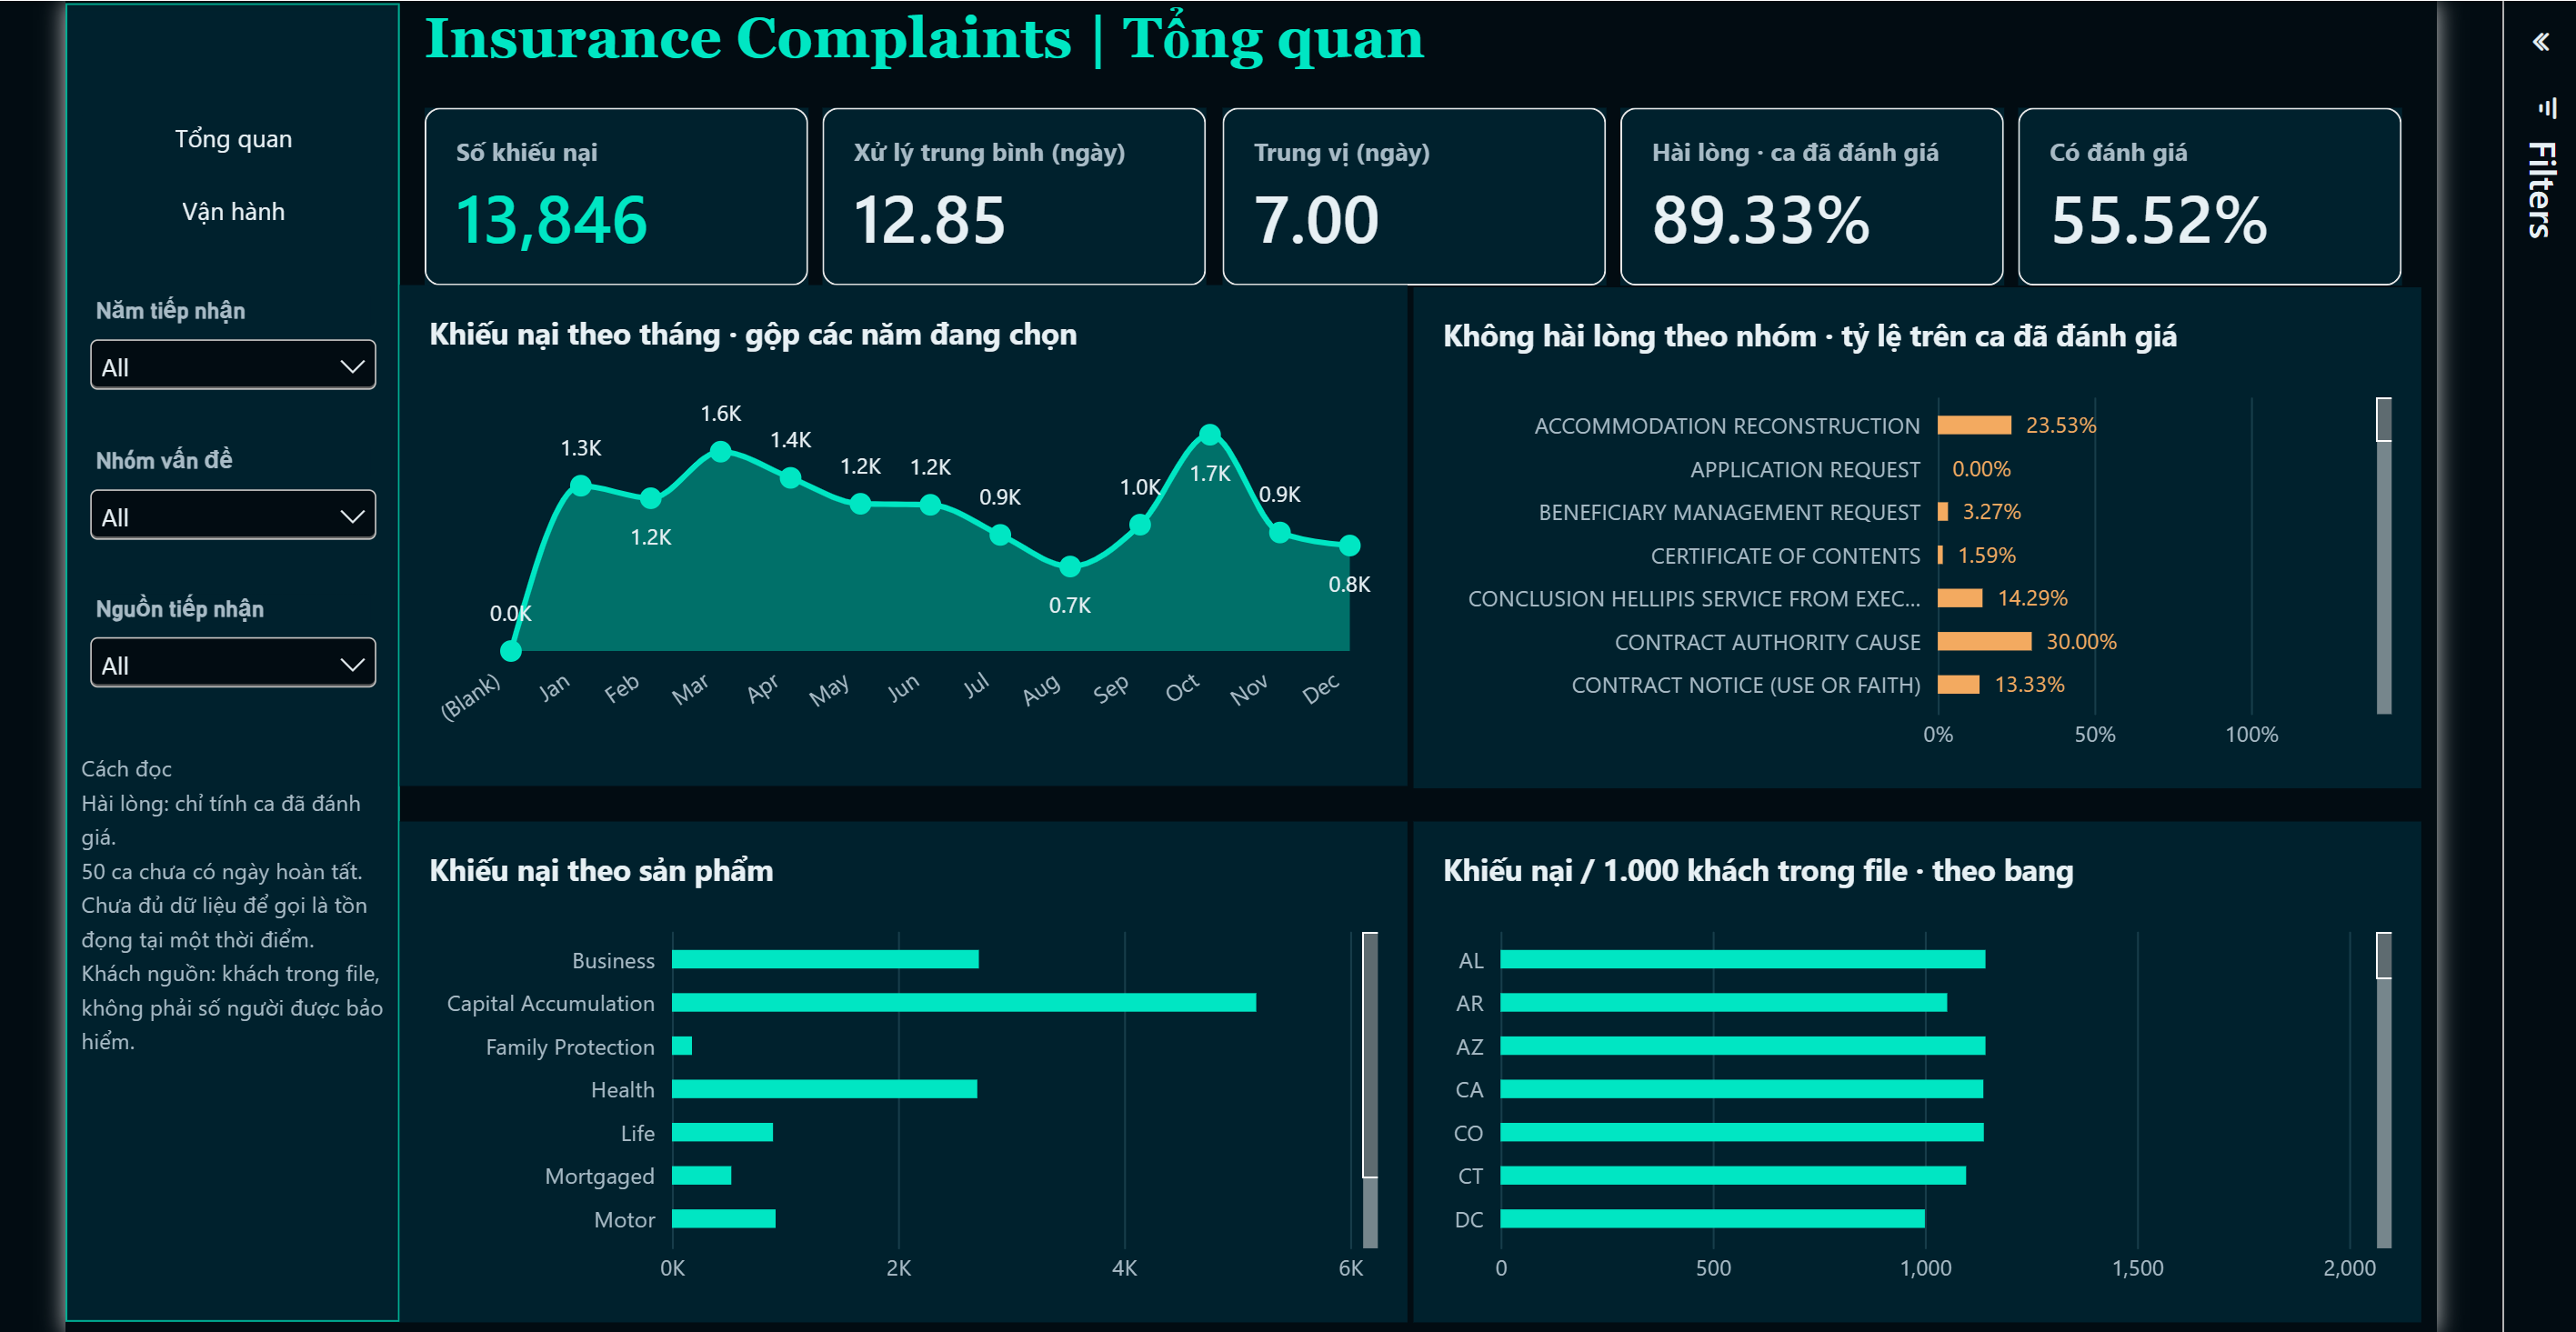
\includegraphics[width=\linewidth]{../phase5/supervisor/after_reopen/Executive Summary.png}
\end{center}
{\small\color{muted}\textbf{Hình 1.} Ảnh canonical sau lưu, đóng và mở lại. Các số trên ảnh dùng dấu phân cách theo giao diện; báo cáo dùng cách viết tiếng Việt.}\par

Trang này trả lời “tình hình chung ra sao?”. Đọc các ô KPI rồi xem nhóm vấn đề, sản phẩm và địa lý. Các ô chọn lấy ra một nhóm hồ sơ; con số sẽ được tính lại theo nhóm đang xem.

\begin{enumerate}
\item Bỏ các lựa chọn để thấy 13.846 hồ sơ. Đọc 89,33\% hài lòng cùng 55,52\% có đánh giá.
\item Chọn năm 2019 và APPLICATION REQUEST: còn 32 hồ sơ, trung bình 0,5 ngày, trung vị 0. Bỏ chọn trước khi so nhóm khác.
\item Chọn CA: có 2.593 ca; thông tin khách nguồn là 2.279. Bỏ chọn để tổng trở về 13.846.
\end{enumerate}

Biểu đồ tháng dùng tên tháng: khi chọn tất cả năm, cùng tháng ở nhiều năm được gộp. Nó không phải chuỗi liên tục theo năm–tháng. Khi chỉ chọn một năm, biểu đồ thể hiện các tháng của năm đó. Dữ liệu 2020 chỉ đến 14/05, nên kỳ năm cuối chưa đầy đủ.

Mở \texttt{TestSkill/pbi/InsuranceOps.pbip} bằng Power BI Desktop. Nếu chuyển máy, kiểm đường dẫn dữ liệu trong hướng dẫn model. Không chạy lại generator cũ chỉ để mở report vì giao diện chỉnh trực tiếp cuối dự án chưa đồng bộ hoàn toàn vào generator.
\evidence{\src{source-images}{F}; \src{source-qa}{B}; \src{source-docs}{C}}
\clearpage

\subsection*{Operation Drill-down — Xem sâu vận hành}
\begin{center}
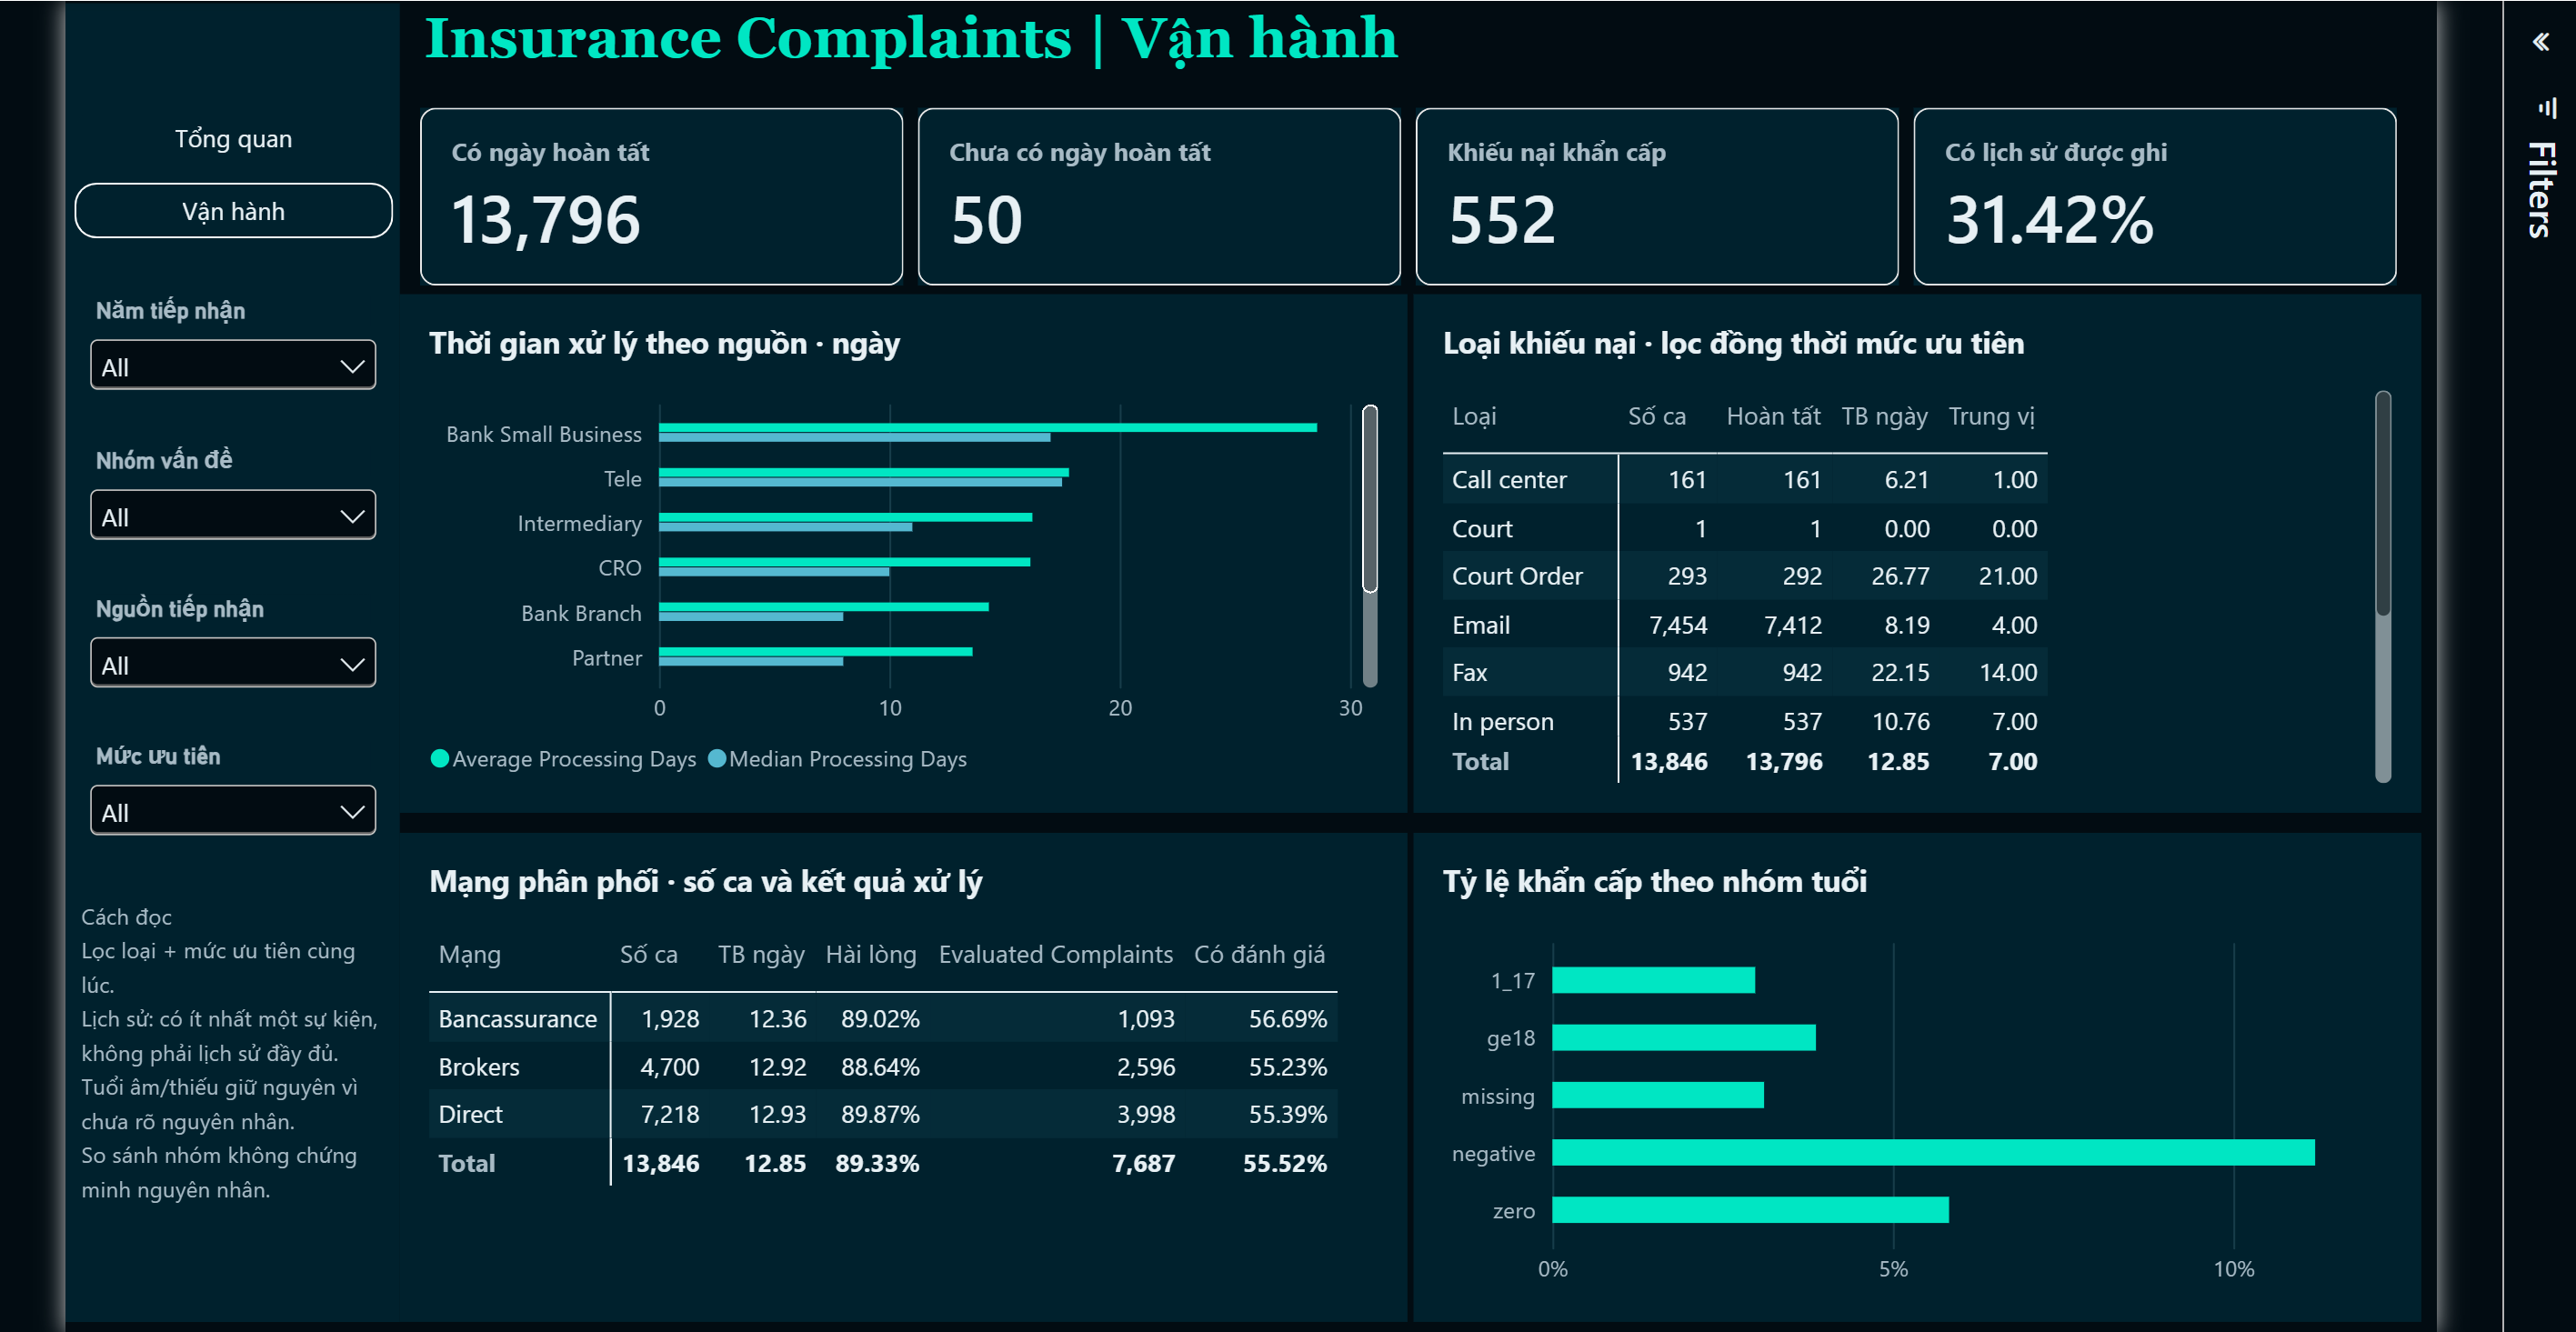
\includegraphics[width=\linewidth]{../phase5/supervisor/after_reopen/Operation Drill-down.png}
\end{center}
{\small\color{muted}\textbf{Hình 2.} Ảnh canonical cùng bản sau mở lại. Mean và median theo Source là hai thanh riêng, không cộng thành tổng.}\par

Trang này giúp xem cùng lúc hình thức, mức ưu tiên, mạng phân phối và nguồn tiếp nhận. Khi đọc biểu đồ, luôn xem số ca trong nhóm. Một nhóm bảy ca không có sức nặng như nhóm hàng trăm ca.

\begin{enumerate}
\item Bỏ chọn trước, rồi chọn Urgent và Email: có 62 ca đã hoàn tất, trung bình 14,23 ngày, trung vị 8,5 ngày.
\item Nhóm này có 6/62 ca có lịch sử, tương đương 9,68\%. Đây là mức có ít nhất một sự kiện, không phải mức đầy đủ lịch sử.
\item Dùng nút Tổng quan/Vận hành để chuyển trang. Trong chế độ chỉnh sửa Desktop có thể cần giữ Ctrl khi bấm. Đã kiểm chuyển trang hai chiều.
\end{enumerate}

\lead{\textbf{Đọc 50 ca thiếu ngày hoàn tất đúng nghĩa:} đây là phần thiếu ngày trong dữ liệu hiện có. Chưa đủ để gọi là hàng đợi tồn đọng tại một mốc. Tương tự, có sự kiện trạng thái chưa đủ để tính thời gian ở từng trạng thái.}

Hai ảnh giúp nhìn sản phẩm; bằng chứng kiểm số, thao tác và lưu/mở lại nằm trong QA cuối. Ảnh tĩnh không chứng minh mọi lựa chọn có thể có đều đã được kiểm.
\evidence{\src{source-images}{F}; \src{source-qa}{B}: Priority Urgent + Type Email, navigation, persistence}
\clearpage

\section{Phương pháp, kỹ thuật và nguồn kiểm chứng}
\subsection*{Kỹ thuật hỗ trợ việc hiểu đúng dữ liệu}
{\small
\begin{tabularx}{\linewidth}{@{}L{4.5cm}Y@{}}
\toprule
\textbf{Thành phần} & \textbf{Vai trò thực tế}\\
\midrule
Excel, Python, CSV, notebook & Đọc nguồn, chuẩn hóa có dấu vết và tính đối chiếu độc lập\\
Power BI, DAX & Tính lại chỉ số theo nhóm được chọn; 22 công thức\\
PBIP, TMDL, PBIR & Lưu dự án, định nghĩa model và định nghĩa giao diện\\
Modeling MCP, Desktop Bridge & Kiểm model và thao tác/quan sát Desktop; hai khả năng riêng\\
PowerShell, hash & Thực thi kiểm, chụp đúng cửa sổ và phát hiện file bị thay đổi\\
OpenCode, Codex & Worker triển khai; supervisor review và tiếp quản dashboard theo quyền đã duyệt\\
\bottomrule
\end{tabularx}}

\subsection*{Cách đếm và kiểm tra}
Model có 16 quan hệ runtime. Bảng khiếu nại dùng mã hồ sơ; bảng lịch sử dùng mã sự kiện. Lọc ngày mặc định theo ngày tiếp nhận; tính theo ngày hoàn tất phải dùng đường ngày riêng. Công thức tỷ lệ dùng đúng mẫu số và giữ điều kiện chọn; giá trị trống không bị biến thành 0 để làm đẹp kết quả.

QA cuối xác nhận 22 công thức/định dạng/nhóm công thức và 22 bản xuất TMDL khớp; 22 phép so baseline sau mở lại khớp; 22 file được bảo vệ không đổi. Có bốn tình huống thử cộng từ đầu năm (YTD), với tám phép so. Đã kiểm CA chọn/xóa, Year × Category ở hai trang, Urgent × Email, chuyển trang và lưu/đóng/mở lại.

Các kiểm tra trên thuộc revision dashboard đã nghiệm thu và được lưu trong QA [B]. Sau nghiệm thu, supervisor ghi nhận một số định nghĩa visual hiện tại khác hash đã lưu; báo cáo dùng ảnh accepted. Lượt viết báo cáo không kiểm lại Power BI hiện tại, nên không mở rộng kết quả QA cũ sang mọi file đang có trên đĩa.

Validator ghi \textbf{0 lỗi, 1 cảnh báo}: không tải được schema \texttt{visualContainer/2.13.0}, nên bỏ qua phần JSON Schema đó. Đây không phải full schema PASS. Không suy từ kiểm cấu trúc sang đúng số, hiển thị hay persistence; các phần này có bằng chứng riêng.

\subsection*{Nguyên tắc DA dùng lại}
\textbf{GIGO:} đầu vào sai có thể làm kết luận sai; vì vậy giữ cờ tuổi bất thường. \textbf{MECE:} chia nhóm không trùng và không thiếu: 6.867 SAT + 820 NSA + 6.159 chưa đánh giá = 13.846. \textbf{KISS:} dùng hai trang cho câu hỏi thực tế, không thêm công nghệ chỉ để đủ mẫu. \textbf{STAR:} kể bối cảnh, việc cần làm, đã làm và kết quả; không kể đề xuất như thành tích.

Skill DA hướng dẫn nối phát hiện → bằng chứng → đề xuất → giới hạn; eli5 giúp giải thích bằng tủ hồ sơ. Chỉ format, thứ tự suy nghĩ và cách kiểm được tái dùng. Nghiệp vụ, KPI, mẫu số, ngưỡng và khuyến nghị của ngành khác phải xác minh riêng.

Dashboard đã nghiệm thu không chứng minh workflow mới thành công ở mọi dự án. Skill vẫn là bản nháp chờ duyệt, chưa cài global. Quy tắc dashboard hai lượt 15 phút đã ghi nhưng chưa được thử trong một handoff mới; nó không phải giới hạn thời gian của báo cáo này.
\clearpage

\subsection*{Chỉ mục nguồn — đường dẫn từ thư mục TestSkill}
\hypertarget{source-index}{}
Các mã [A]–[F] trong báo cáo dẫn tới chỉ mục này. Giữ TEX trong \texttt{reports/project\_report/} và giữ hai ảnh canonical tại vị trí hiện có để có thể biên dịch lại. Đường dẫn bên dưới trỏ tới artifact thực; PDF giữ ảnh nhúng để xem độc lập.

\begin{description}[style=nextline,leftmargin=0pt,labelindent=0pt,labelwidth=0pt,itemsep=8pt]
\item[\textcolor{teal}{[A] Phân tích tổng hợp canonical}\label{source-analysis}]
\href{../../Log/phase5/analysis.json}{\nolinkurl{Log/phase5/analysis.json}}\par
Nguồn cho KPI tổng và các nhóm Q1–Q10 có dữ liệu. Các section của JSON được nêu gần từng kết luận. Q8 thiếu dữ liệu, không tạo số thay thế.
\item[\textcolor{teal}{[B] QA cuối và nghiệm thu dashboard}\label{source-qa}]
\href{../../Log/phase5/supervisor/qa_final.json}{\nolinkurl{Log/phase5/supervisor/qa_final.json}}\par
Chứa modelChecks, uiChecks, validation, revisionHashes, evidenceHashes, limitations và humanAcceptance. Là nguồn trạng thái cuối, thay các checkpoint lịch sử.
\item[\textcolor{teal}{[C] Báo cáo, hướng dẫn sử dụng và giải thích DA}\label{source-docs}]
\href{../../docs/06_project_report.md}{\nolinkurl{docs/06_project_report.md}}\par
\href{../../docs/05_insights_and_report.md}{\nolinkurl{docs/05_insights_and_report.md}}\par
\href{../../docs/07_da_explained.md}{\nolinkurl{docs/07_da_explained.md}}\par
Giải thích kết quả, giới hạn và cách dùng dashboard; đề xuất vẫn chưa triển khai.
\item[\textcolor{teal}{[D] Nguồn, chất lượng và chuẩn hóa}\label{source-data}]
\href{../../data/insurance_complain.xlsx}{\nolinkurl{data/insurance_complain.xlsx}}; đề bài trong \texttt{data/Đề bài.docx}\par
\href{../../docs/01_data_understanding.md}{\nolinkurl{docs/01_data_understanding.md}}\par
\href{../../docs/02_transformation.md}{\nolinkurl{docs/02_transformation.md}}\par
Tài liệu kỹ thuật giữ grain, kỳ dữ liệu, quy tắc bảo toàn và phần thiếu. Chỉ dùng nội dung có bằng chứng phù hợp; trạng thái cũ trong tài liệu không thay QA cuối.
\item[\textcolor{teal}{[E] Model và registry công thức}\label{source-method}]
\href{../../docs/03_semantic_model.md}{\nolinkurl{docs/03_semantic_model.md}}\par
\href{../../docs/04_measures.md}{\nolinkurl{docs/04_measures.md}}\par
Định nghĩa liên kết, ngày lọc, công thức, mẫu số và cách xử lý nhóm rỗng.
\item[\textcolor{teal}{[F] Hai ảnh accepted sau mở lại}\label{source-images}]
\href{../phase5/supervisor/after_reopen/Executive Summary.png}{Executive Summary.png}\par
\href{../phase5/supervisor/after_reopen/Operation Drill-down.png}{Operation Drill-down.png}\par
Trong \texttt{reports/phase5/supervisor/after\_reopen/}; hash ảnh được lưu ở nguồn [B]. Không sao chép hoặc sửa ảnh nguồn.
\end{description}

\lead{\textbf{Giới hạn cần giữ khi chia sẻ:} phát hiện mô tả bộ dữ liệu hiện có. Chưa chứng minh nguyên nhân, hiệu quả can thiệp, rủi ro trên dân số bảo hiểm, thời gian ở trạng thái, cloud publish hoặc SLA vận hành.}
\end{document}
